\documentclass[SRC.tex]{subfiles}

\begin{document}
	\subsection{Termodynamiske processor}
	Idealgasligningen er en ligning, som kan anvendes til at beskrive sammenhængen mellem
	\textit{tryk}, \textit{volumen}, \textit{stofmængde} og \textit{temperatur} for en ideal 
	gas og derved dens tilstand. Den kan afbildes rent matematisk som
	\begin{equation}
	p \cdot V = n \cdot R \cdot T
	\label{eq:idealgasligningen}
	\end{equation}
	hvor \(p\) er gassens tryk, \(V\) er gassenes volumen, \(n\) er stofmængden, \(R\) er gaskonstanten
	og har værdien \(\SI{8.314}{\joule\per (\mole\cdot\kelvin)} \) og \(T\) er temperaturen angivet i 
	Kelvin. Mere specifikt gør ligningen sig 
	gældende for ideale gasser, hvilket betyder, at der antages at gasmolekylerne kolliderer 
	total elastisk imellem hinanden, altså at der ikke går nogen energi tabt ved sammenstød af 
	molekyler. Hvis man begynder at ændre på to af de resterende faktorer ved en indespæret gas, 
	som har en konstant stofmængde, så vil den tredje variable indstille sig, så den overholder
	idealgasligningen. Denne indstilling fra et stadie til et andet kaldes for en \textit{proces}. 
	Generelt for alle processorer gælder det, at temperaturen direkte korrelerer til ændringen af 
	en given gas' indre energi, som er et begreb for molekylernes kinetisk energi og indbyrdes 
	kræfter i gassen. Dette kan illustreres ved
	\begin{equation}
	\Delta E_i = n \cdot c_{\text{mV}} \cdot \Delta T
	\label{eq:2}
	\end{equation}
	hvor \(\Delta E_i\) er den indre energi i gassen, \(n\) er stofmængdekoncentrationen i mol, 
	\(c_{\text{mV}}\) er den specifikke molære varmekapacitet ved et konstant volumen. (Holck og Kraaer, 2009)
	
	\subsubsection{Isokor process} 
	Hvis en gas indespæret med konstant volume oplever en varmetilførsel, så vil 
	gassens tryk variere alt efter, om der er en positiv eller negativ varmetilførsel. En sådan
	process, hvor volumenet holdes konstant kaldes en \textit{isokor} proces. Arbejdet som en 
	gas under en isokor proces udfører kan beregnes ved som følgende  
	\begin{equation}
	A = p \cdot \Delta V.
	\label{eq:3}
	\end{equation}
	Idet volumenet i en isokor proces er konstant, så er volumeændringen \(\Delta V\) lig nul, og derved vil arbejdet
	også være lig nul, da gassen ikke kan 'skubbe' på omgivelserne ved at udvide sig ligeledes er 
	omgivelsernes arbejde på gassen lig nul.
	\begin{equation}
	A = 0
	\end{equation}
	Formlen for at beregne den nødvendige mægnde varme, \(Q\), som skal tilføres til gassen under 
	en isokor proces, kan findes ved den tidligere nævnte formel \eqref{eq:2}
	\begin{equation}
	Q = n \cdot n_{\text{mV}} \cdot \Delta T
	\end{equation}
	(Holck og Kraaer, 2009)
	
	\subsubsection{Isobar proces}
	Forskellen fra en isokor til en isobar process er, at trykket 
	holdes konstant fremfor volumenet som i det forrige. Ved
	denne proces kan det udførte arbejde på gassen, altså 
	omgivelsernes arbejde, findes ved
	\begin{equation}
	A = -p \cdot \Delta V
	\end{equation}
	som er den samme som ligning \eqref{eq:3} bortset fra at
	der er introduceret et negativt fortegn. Dette er gjort fordi det er arbejdet fra omgivelserne 
	på gassen, der betragtes. Arbejdet vil kun være positivt, når gassen komprimeres, idet det 
	vil resultere i en negativ volumeændring. 
	
	Den tilførte varme, \(Q\), som skal tilføres gassen for at 
	resultere i temperaturændrigen \(\Delta T\) kan findes ved
	\begin{equation}
	Q = n \cdot (c_{\text{mV}} + R) \cdot \Delta T
	\end{equation} 
	hvor man indfører en special varmekapacitet, som kaldes \textit{den specifikke molære varmekapacitet ved konstant tryk} der denoteres som \(c_{\text{mp}}\). Denne varmekapacitet anvendes ved en isobar proces og er defineret som
	\begin{equation}
	c_{\text{mp}} = c_{\text{mV}} + R
	\end{equation}
	Så beregnes den tilførte varme, \(Q\), nu ved
	\begin{equation}
	Q = n \cdot c_{\text{mp}} \cdot \Delta T
	\end{equation}
	(Holck og Kraaer, 2009)
	\subsubsection{Isoterm proces}
	En isoterm proces er en proces, hvor temperaturen holdes konstant. 
	Derfor må gassens indre energi også være konstant, da den direkte 
	indikerer temperaturen på gassen, ligesom i formel \eqref{eq:2}.
	Hvis der tilføres eller fjernes varme under en 
	isoterm proces, så må der på tilsvarende vis udføres et arbejde for
	at komme af med den overskydne varme og holde temperaturen konstant,
	og hvis der fjernes varme, så må der tilføres et arbejde på gassen
	for at holde temperaturen konstant. Ved en isoterm proces kan det 
	arbejde, som omgivelserne skal udføre på gassen beregnes ved
	\begin{equation}
	A = -n \cdot R \cdot T \cdot \ln\left(\frac{V_{\text{slut}}}{V_{\text{start}}}\right)
	\label{eq:10}
	\end{equation}
	Det arbejde, som udføres på en gas under en isoterm proces, skal 
	udlignes af den tilførte varme \(Q\) for at temperaturen kan forblive
	konstant, deraf har vi
	\begin{equation}
	Q = n \cdot R \cdot T \cdot \ln\left(\frac{V_{\text{slut}}}{V_{\text{start}}}\right)
	\label{eq:11}
	\end{equation}
	Den eneste forskel på ligning \eqref{eq:10} og \eqref{eq:11} er fortegnet,
	hvilket bevidner, at de to er modsatte.
	
	Endvidere, hvis en isoterm proces plottes i et \textit{pV}-diagram, så 
	vil den afbilde en hyperbel. Netop da, hvis man isolerer \(p\) og \(V\)
	i idealgasligningen \eqref{eq:idealgasligningen}, så følger det
	\begin{equation}
	p = n \cdot R \cdot T \cdot \frac{1}{V}
	\end{equation}
	Netop da den plottes i et \textit{pV}-diagram, hvor førsteaksen er volumenet,
	\(V\), så vil trykket \(p\) aftage asympotisk som volumenet stiger. 
	\subsubsection{Adiabatisk proces}
	En adiabatisk proces er en proces, hvorved der ikke udveksles varme med 
	omgivelserne. Denne proces finder eksempelvis sted i en dieselmotor, hvor dens 
	stempel, som komprimerer en blanding af dieselolie og luft så hurtigt og kraftigt,
	at gassen ikke har tid til at afgive varme til hverken cylindreret eller stemplet. Så alt arbejdet går til at få temperaturen på gassen til at stige. Altså sker der en stigning i indre energi, hvilket betyder at 
	\begin{equation}
	Q = 0
	\end{equation}
	Med andre ord, så forekommer der ingen varmetilførsel, hverken til eller fra gassen. Netop da 
	alt det udførte arbejde bliver omdannet til indre energi i gassen. Heraf kan
	følgende opstilles med formel \eqref{eq:2}
	\begin{equation}
	A = n \cdot c_{\text{mV}} \cdot \Delta T 
	\end{equation}
	Følgende gælder for en adiabatisk proces
	\begin{equation}
	p \cdot V^\gamma = k,\quad \text{det betyder at}\ p_1 \cdot V_1^\gamma= p_2 \cdot V_2^\gamma
	\end{equation}
	og 
	\begin{equation}
	T \cdot V^{\gamma-1} = k,\quad \text{det betyder at}\ p_1 \cdot V_1^{\gamma-1}= T_2 \cdot V_2^{\gamma-1}
	\end{equation}
	hvor \(k\) er en konstant og \(\gamma\) kaldes
	for adiabatkonstanen eller varmefyldeforholdet, der er defineret som
	\begin{equation}
	\gamma = \frac{c_{\textrm{mp}}}{c_{\textrm{mV}}}
	\end{equation}
	(Holck og Kraaer, 2009)
	\subsection{Kredsprocesser}
	Alle ovenstående termodynamiske processor kan kombineres til at danne
	en såkaldt \textit{kredsproces}. En kredsproces består af op til flere 
	forskellige termodynamiske processorer i en vilkårlig rækkefølge, som en gas i 
	et lukket system ville opleve. Det definerende ved en kredsproces er at det fungere som en kreds, altså at efter alle påvirkninger
	fra de forskellige termodynamiske processor, så vender gassen tilbage i dens starttilstand med
	samme tryk, temperatur og volume. Udledningsvist, betyder dette, at ændringen 
	i gassens indre energi er nul, da den starter og slutter samme sted. Derfor gælder følgende for en kredsproces
	\begin{equation}
	\Delta E_\text{i} = 0
	\end{equation} 
	\subsubsection{Arbejde i kredsprocessor}
	For at få et overblik over en kredsproces, så kan det være fordelagtigt at 
	integne dem i et \(pV\)-diagram, hvor førsteaksten er volume, \(V\) og 
	andenaksen er trykket, \(p\), dette er gjort på figur \ref{fig:csm044pvdiagram235px7d08cd8d72}
	\begin{figure}[h!]
		\centering
		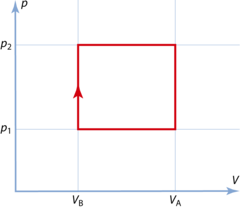
\includegraphics[scale=0.5]{Billeder/csm_044_PV_diagram_235px_7d08cd8d72}
		\caption{simpel kredsproces indtegnet i et \(pV\)-diagram. Kilde: \url{https://orbithtxa.systime.dk/?id=281}}
		\label{fig:csm044pvdiagram235px7d08cd8d72}
	\end{figure}
	
	I kredsprocessen i figur \ref{fig:csm044pvdiagram235px7d08cd8d72} ses det, at pilen indikerer, at omløbsretningen er med uret, derfor udføres der
	først en isokor opvarmning, så en isobar ekspansion, så en isokor afkøling og
	endelig en isobar kompression, så den er tilbage til starttilstanden. I 
	kredsprocesson udføres der et arbejde ved to isobare processor. Først ved
	den isobare ekspansion, hvor gassen udvider sig og derved udfører et arbejde
	på omgivelserne, derefter udfører omgivelserne et arbejde på gassen idet den 
	komprimeres ved den isobare kompression. Bemærk, at de to stykker arbejde der
	udføres, ikke er lige store, idet den isobare ekspansion finder sted ved et meget
	højere tryk end den isobare kompression. Nettoarbejdet for enhver kredsproces er
	lig det areal, som determodynamiske processor afgrænser i \(pV\)-diagrammet. 
	
	Hvis kredsprocessens gas' omløbsretning forløber med uret i \(pV\)-diagrammet, 
	så udfører gassen et positivt arbejde på omgivelserne, ligesom i eksemplet, 
	hvor gassens arbejde er større end omgivelsernes arbejde på gassen, derfor vil 
	nettoarbejdet være positivt. Dermed så modtager gassen varme og 
	udførerer et mekanisk arbejde - en sådan maskine benævnes som en kraftvarmemaskine. Hvorimod hvis gassen forløber mod uret, så udfører 
	omgivelserne et positivt arbejde på gassen. Udfra termodynamikkens første 
	hovedsætning samt at i en kredsproces gælder \(\Delta E_\text{i} = 0\), kan 
	følgende opstilles
	\begin{equation}
	A_{\text{gas}} = Q_{\text{tilført}} - Q_{\text{afgivet}}
	\end{equation} 
	hvor \(A_{\text{gas}}\) er gassens nettoarbejde på omgivelserne, 
	\(Q_{\text{tilført}}\) er den varme, som omgivelserne tilfører gassen i 
	kredsprocessens forløb og \(Q_{\text{afgivet}}\) er den varme, der afgives 
	til omgivelserne fra gassen. (Holck og Kraaer, 2009) (Systime) 
	
	\subsection{EuroDish}
	EuroDish er en maskine, som udvikles i projektet EnviroDish. Maskinen består
	af en parabolsk formet koncentrator, som koncentrerer solens lys i et brændpunkt. 
	I brændpunket er monteret en Stirling motor, som er koblet til en el-generator,
	der omdanner Stirling motorens mekaniske arbejde til el, der kan sendes ud til 
	elnettet eller anvendes lokalt. For at udnytte solens energi bedst muligt, så er
	selve monteringsanordningen konfigureret sådan, at den ved instruktioner fra en 
	sensor kan følge solens bane på himlem og derved altid være optimalt placeret i forhold til solen. Se figur \ref{fig:744-9} for et billede af en 
	monteret EuroDish. (promes, u.d.) 
	\begin{figure}[h]
		\centering
		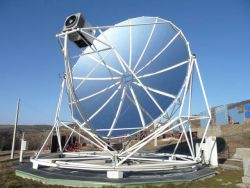
\includegraphics[scale=0.6]{Billeder/744-9}
		\caption{Billede af en monteret EuroDish kilde: (promes, u.d.) }
		\label{fig:744-9}
	\end{figure}
\end{document}